\begin{frame}{Climbing Multistrings: Finding Stationary Points, Ala$_3$}
\begin{tikzpicture}
\pcuad{\textwidth}{\textheight}
\path(hl)
    ++(0,-1) node(img1)[anchor=south]{
        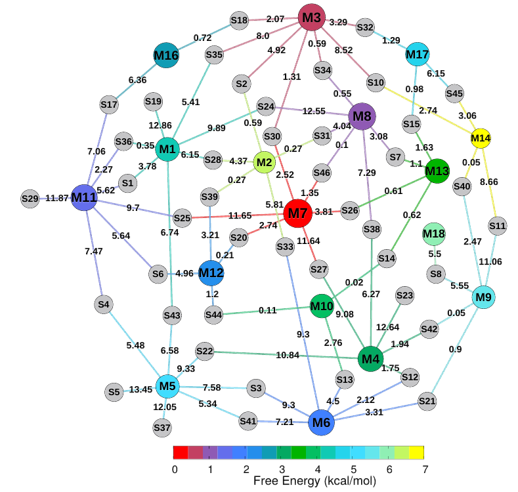
\includegraphics[height=0.6\textheight]{ala3network.png}
    }
    ++(0.33\textwidth,0.5) node(img2)[anchor=center]{
        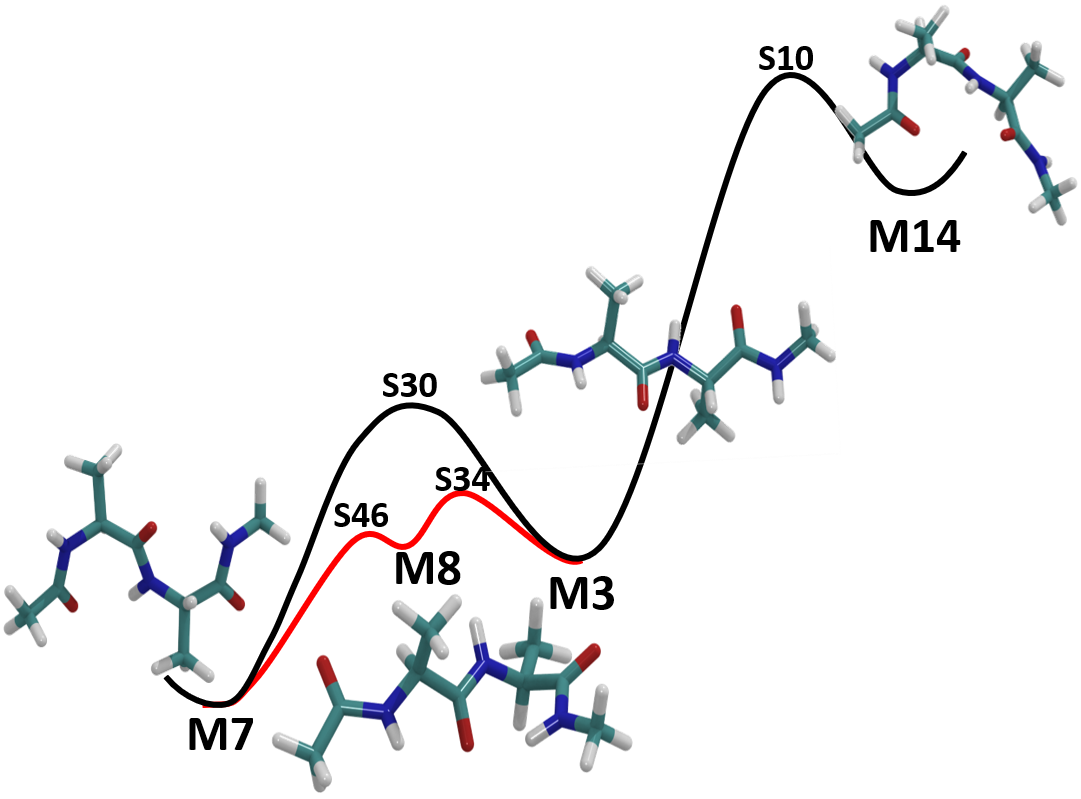
\includegraphics[height=0.7\textheight]{ala3pathway.png}
    };
\path(se)
    ++(0,0.5) node(att)[anchor=east]{
        {\tiny \textcolor{blue!80!black}{G. Shrivastav and CFA, {\it J Chem Phys} 2019 {\bf 151}:124112}}
    };
\end{tikzpicture}
\end{frame}
